\documentclass[11pt]{article}
\usepackage[T1]{fontenc}
\usepackage{lmodern}
\usepackage[margin=1in]{geometry}
\usepackage{amsmath,amssymb,amsthm,mathtools}
\usepackage{microtype,booktabs,longtable,array,enumitem}
\usepackage[dvipsnames]{xcolor}
\usepackage{graphicx,fancyhdr,listings}
\usepackage[most]{tcolorbox}
\usepackage{hyperref}
\hypersetup{colorlinks=true,linkcolor=MidnightBlue,citecolor=MidnightBlue,
 urlcolor=MidnightBlue,pdftitle={Minimum Envelopes and Complete Normal-Surface Sectors}}
\setlength{\emergencystretch}{2em}
\setlist{itemsep=3pt,topsep=5pt}
\pagestyle{fancy}\fancyhf{}
\fancyhead[L]{\small Minimum envelopes for normal-surface sectors}
\fancyhead[R]{\small ProveIt research continuation}
\fancyfoot[C]{\thepage}
\setlength{\headheight}{14pt}
\newtheorem{theorem}{Theorem}[section]
\newtheorem{lemma}[theorem]{Lemma}
\newtheorem{corollary}[theorem]{Corollary}
\newtheorem{proposition}[theorem]{Proposition}
\theoremstyle{definition}
\newtheorem{definition}[theorem]{Definition}
\newtheorem{example}[theorem]{Example}
\theoremstyle{remark}
\newtheorem{remark}[theorem]{Remark}
\newcommand{\R}{\mathbb R}\newcommand{\Q}{\mathbb Q}
\newcommand{\Z}{\mathbb Z}\newcommand{\N}{\mathbb N}
\newcommand{\cone}{\mathcal C}\newcommand{\stdcone}{\mathcal K}
\newcommand{\lift}{\mathcal E}\newcommand{\poly}{\operatorname{poly}}
\newcommand{\supp}{\operatorname{supp}}
\newcommand{\rank}{\operatorname{rank}}
\newcommand{\conv}{\operatorname{conv}}
\newcommand{\Ker}{\operatorname{ker}}
\newcommand{\lin}{\operatorname{span}}
\lstset{basicstyle=\small\ttfamily,breaklines=true,columns=fullflexible,
 keepspaces=true,frame=single,rulecolor=\color{black!15},
 backgroundcolor=\color{black!2},showstringspaces=false}

\title{\vspace{-1.0cm}\textbf{Minimum Envelopes and Complete\\Normal-Surface Sectors}\\[0.35em]
\large Linear ray bounds, exact enumeration, and independent coverage certificates}
\author{A research continuation for the ProveIt project}
\date{9 October 2026}

\begin{document}
\maketitle
\begin{abstract}
The current ProveIt arrangement backend forms every pairwise equality between
triangle potentials and then rejects directions that fail a standard-coordinate
extremality test. We identify the smaller geometric object that is actually
needed: the common subdivision on which the per-vertex minimum potentials are
linear. An anchored cell of this subdivision is linearly isomorphic to a
coordinate face of the standard matching cone. Consequently its rays are
already standard extreme rays; a subsequent rank filter is unnecessary.

For a compatible sector with $k$ allowed quadrilateral types and matching
nullity two, projective normalization reduces the problem to affine lower
envelopes on a closed interval. All non-link standard rays are exactly its
endpoints and the genuine changes of these envelopes. If $p$ triangle classes
and $g$ nontrivial vertex groups survive contraction, their number satisfies
$N\le p-g+2\le 3k+4$. Empty and one-ray cones are handled exactly. Once the
sector kernel is constructed, the implementation uses
$O(1+k+kp+p\log(p+1)+N(t+p+k))$ exact operations to emit full coordinates,
where $t$ is the number of tetrahedra. This simplifies to $O(tk)$ for
$k\ge1$, with native coordinate validation charged separately; bit
complexity remains polynomial. We also prove a linear arithmetic
verification rule for envelope coverage using one slope-bracket witness per
source line. The supplied checker reconstructs the matching model independently
and never calls a ray producer.

The package contains an opt-in integration with the maintained implementation,
source code, adversarial and independent tests, frozen and fresh Regina
comparisons, paired measurements on actual triangulations, and reproducible
certificates. The result advances complete candidate enumeration in supplied
low-dimensional sectors. A complete sector-family theorem and global control
of topology transformations remain necessary for a general
$n^{O(\log n)}$ unknot recognizer.
\end{abstract}

\begin{tcolorbox}[colback=MidnightBlue!4,colframe=MidnightBlue!45,
 title={Reading the claims}]
The fan correspondence, the linear ray bound, and the coverage theorem are
proved below. Runtime measurements are experiments on the declared queries.
The global recognition corollary is conditional on explicitly stated discovery
and coverage assumptions. No general quasi-polynomial recognition theorem is
claimed.
\end{tcolorbox}
\clearpage
\tableofcontents
\newpage

\section{The bottleneck and the contribution}
\label{sec:introduction}

The input to the local problem is a finite triangulation and a specified
compatible choice of allowed quadrilateral types. The desired output is the
\emph{complete} list of standard-coordinate extreme normal rays in that
sector, with pure vertex links omitted. This list supports subsequent choices
of compressing discs, components, or other normal surfaces. A first
positive-Euler witness is a weaker query and must not be substituted for it
when comparing algorithms.

The repository snapshot used here is commit
\texttt{66098968e88bba797143ac1bf7ad0ac4c5f697df}. At that revision,
\texttt{fastunknot/normal\_sector.py} contracts zero-labelled triangle matching
edges, constructs a finite consistency matrix, and offers an arrangement method
and a support-enumeration method. The arrangement method restricts every
coordinate hyperplane and every pairwise triangle-potential equality to the
quadrilateral matching space. It enumerates intersections of these hyperplanes,
lifts nonnegative directions, and tests whether their positive standard support
has a one-dimensional kernel. These steps are exact, but most potential
equalities need not describe a minimum. The construction therefore over-refines
the geometry before paying for its correction.\cite{repo,report57}

Three recent incoming packages were inspected in addition to the maintained
code. The dual-certificate package replaces some positive-Euler searches by
anchor linear programs and explicitly asks for certified removal of redundant
minimum-potential choices. The support-sensitive package concerns the cost of
observing supplied normal vectors. The transport package constructs and checks
topological changes and ordered boundary data. The present contribution is a
complete low-dimensional enumeration method, answering a tractable part of the
minimum-potential question while retaining all standard rays.\cite{incomingdual,
incomingsupport,incomingtransport}

\subsection{What is new in this continuation}

The main mathematical statement is a coordinate-face correspondence, valid in
all dimensions. It explains precisely which subdivisions preserve standard
extremality. Its two-dimensional specialization gives an exact output list and
a linear bound; it does not merely bound the number of directions tried by a
heuristic. A second structural argument combines the cycle rank of the
contracted triangle graph with quadrilateral matching rank to sharpen the
initial $4k+2$ bound to $3k+4$.

The implementation follows these proofs. It never constructs pairwise
potential hyperplanes, never calls the supported-rank filter, and projects
triangle potentials only once. The independent checker rebuilds an
uncontracted source model from matching equations. A checked slope bracket
proves that each original line is above the claimed envelope throughout the
interval. Thus a completeness claim can be checked without regenerating the
old arrangement or invoking the new producer.

\subsection{Relation to established work}

Canonical extension from quadrilateral coordinates, removal of vertex links,
and general conversion to the standard solution set are established parts of
normal-surface theory. Burton gives a canonical extension algorithm and a
general conversion algorithm; his work also explains why standard and
quadrilateral vertex lists can differ.\cite{burtonconversion} Affine lower
envelopes and their relation to planar convex hulls are classical computational
geometry.\cite{cgalenvelopes} The contribution here is a proved specialization
of canonical conversion, its graph-sensitive count, and its exact integration
and validation against the previous implementation. The literature examination
does not establish priority for every isolated lemma.

Global bounds obtained from maximal admissible faces provide related context.
The closed connected manifold hypotheses in Burton's asymptotic bounds must
be retained; those bounds are not transferred here to finite knot exteriors
with boundary.\cite{burtonfaces}

Linear-programming feasibility and quadrilateral branching also have extensive
precedents. Burton and Ozlen study fast branching and tree traversal for
normal-surface decisions.\cite{burtonozlen,treetraversal} We do not describe
those general ideas as new. Nor does the present result settle a general
output-polynomial conversion question: the bounded-dimensional case is the
essential restriction.

Lackenby's July 2026 preprint supplies a hierarchy-based incompressibility
algorithm and analyses hierarchy constructions. Its introduction leaves
speed-up to future work; it is not a proved running-time specification for the
announced quasi-polynomial goal.\cite{lackenby2026} The implementation developed
here addresses one local part of a prospective certified hierarchy or surface
search.

\section{Finite normal matching and compatible sectors}
\label{sec:setting}

Let $\mathcal T$ be a finite triangulation of a compact three-manifold, with
$t$ tetrahedra. Face identifications and boundary faces are part of the input.
The native validation used by the implementation checks its accepted
finite-manifold schema before any normal-coordinate claim is made. A
triangulation supplied to this API is not, solely by being supplied, a
certificate that it is the exterior of a particular knot diagram.

Each tetrahedron has four triangular and three quadrilateral normal disc
types. A standard coordinate vector consists of their nonnegative counts.
Vertices and opposite faces are numbered $0,1,2,3$. Quadrilateral types
$0,1,2$ avoid the opposite edge pairs $01|23$, $02|13$, and $03|12$,
respectively. A face-pairing permutation lists the images of vertices
$0,1,2,3$ in that order.
For a face and an arc type, matching takes the form
\begin{equation}
 x_a+q_i=x_b+q_j,
 \label{eq:matching}
\end{equation}
with a missing or forbidden quadrilateral contribution interpreted as zero.
These are finite matching equations. We do not replace them by a possibly
different system for spun surfaces in an ideal triangulation.

\begin{definition}[Compatible allowed sector]
A sector $\Sigma$ is a set of $k$ pairs $(\tau,j)$, containing at most one
quadrilateral type for each tetrahedron. Quadrilaterals outside $\Sigma$ are
forced to zero. The allowed coordinates may themselves vanish. Thus $k$ is
the number of \emph{allowed} types, not necessarily the positive support of
an output ray.
\end{definition}

Write $q\in\R^k$ for the allowed quadrilateral coordinates and $x$ for
triangle coordinates. The standard sector cone $\stdcone_\Sigma$ consists of
the nonnegative solutions of the finite matching equations. It is a
coordinate face of the unrestricted nonnegative standard matching cone:
forcing forbidden quadrilaterals to zero imposes coordinate-face equations.
Hence its extreme rays are exactly the unrestricted standard extreme rays
that lie in the sector. This observation justifies comparison with a complete
Regina standard-ray list filtered by allowed types.

Two concepts of dimension must be kept distinct. A rational linear matching
space can have dimension two while its nonnegative part is empty apart from
zero, or is only one-dimensional. The implementation first computes the
rational matching nullity and then determines the actual feasible section.

\begin{table}[ht]
\centering
\begin{tabular}{@{}>{$}l<{$}p{10.9cm}@{}}
\toprule
t & Number of tetrahedra in the supplied finite triangulation.\\
k & Number of allowed quadrilateral types, with $k\le t$.\\
A & Triangle-graph cycle consistency matrix on the $k$ coordinates.\\
d & Rational matching nullity $\dim\Ker A$.\\
a & Number of matching edges with a nonzero quadrilateral label.\\
p & Number of retained triangle classes after zero-label contraction.\\
g & Number of retained vertex groups; each retained group has at least two classes.\\
N & Number of emitted non-link standard extreme rays.\\
H & A bound on binary sizes of rational numbers in the post-kernel computation.\\
\bottomrule
\end{tabular}
\caption{Notation. Vertex-link factors removed by the compiler contribute
neither to $p-g$ nor to the non-link ray count.}
\end{table}

\section{The triangle graph, potentials, and encoded size}
\label{sec:graph}

Construct a graph whose vertices are tetrahedron corners. Every face matching
equation connects its two triangle corners. Orient the edge so that
\begin{equation}
 x_b-x_a=\eta_e\cdot q,
 \qquad \eta_e\in\Z^k.
 \label{eq:edge}
\end{equation}
Loops and repeated edges are allowed. The connected components of this graph
are the global vertices of the triangulation. On a spanning forest, propagate
integral vector potentials $\ell_c$ so that a candidate solution has
\begin{equation}
 x_c=\alpha_v+\ell_c(q),\qquad c\in G_v.
 \label{eq:potential}
\end{equation}
The remaining edges give consistency equations $Aq=0$. An edge with zero
label forces its two triangle coordinates to agree identically and can be
contracted. The maintained compiler performs this contraction before building
its reduced standard cone.

At a vertex whose corners all contract to one class, that class is a free
vertex-link factor and can be omitted from the retained kernel. The other
classes form groups $G_v$ of sizes at least two. There are $p$ such classes
and $g$ such groups. Formula~\eqref{eq:potential} remains valid on them.

\begin{lemma}[Label and forest counts]
\label{lem:graphcounts}
For a sector with $k$ allowed types,
\begin{equation}
 a\le4k,\qquad p-g\le a,\qquad
 \rank A\le a-(p-g).
 \label{eq:graphcounts}
\end{equation}
Consequently, with $d=k-\rank A$,
\begin{equation}
 p-g\le a-k+d\le3k+d.
 \label{eq:sharpergraph}
\end{equation}
\end{lemma}

\begin{proof}
An allowed quadrilateral has four sides, one on each tetrahedron face. Each
side can contribute to at most one matching-edge label. Therefore the number
of edges with a nonzero label is at most the total $4k$ incidences. Cancellations,
boundary faces, and repeated identifications can only lower this count.

Before deletion, each global-vertex triangle graph is connected. Delete the
nonzero-labelled edges and contract the connected components of the remaining
zero-labelled graph. If there are $c_v$ resulting vertices at a global
vertex, a spanning tree of its active quotient graph contains $c_v-1$ edges.
The total forest size is $\sum_v(c_v-1)=p-g$, including zero contributions
from singleton groups. This gives the second inequality.

There are exactly $a-(p-g)$ edges outside a spanning forest, counting loops.
After forest potentials are assigned, one cycle consistency equation for each
of those edges suffices. The rank of the consistency matrix cannot exceed the
number of equations in this presentation. Substituting $\rank A=k-d$ proves
\eqref{eq:sharpergraph}.
\end{proof}

\subsection{A useful inherited coordinate bound}

The following argument reestablishes the support-kernel height bound used by
the existing implementation. It is included to make binary complexity
explicit, rather than interpreting normal-disc multiplicity as input length.
The bound itself belongs to the preceding sector work.\cite{report57}

\begin{lemma}[Mixed-column minor bound]
\label{lem:height}
Every primitive nonnegative standard extreme ray in a sector with $k$ allowed
quadrilateral types has all retained coordinates at most $4^k$. Expanding
contracted triangle classes back to tetrahedron corners preserves this bound.
\end{lemma}

\begin{proof}
Write the retained standard matching matrix in triangle and quadrilateral
blocks. The triangle block is the transpose of an oriented graph incidence
matrix, possibly with zero rows from loops. Every square minor of that block
is $0$, $1$, or $-1$. Each quadrilateral column has total absolute sum at most
four, since its entries arise from at most four quadrilateral sides.

Expand a square minor along its $r\le k$ quadrilateral columns. The remaining
triangle minor has absolute value at most one. The sum of the absolute
expansion terms is bounded by the product of the column $\ell^1$ norms, so
the original minor has absolute value at most $4^r\le4^k$.

Let an extreme ray have positive support of size $s$. The matching matrix
restricted to this support has rank $s-1$. Choose $s-1$ independent rows.
Its signed maximal minors give a nonzero integral kernel vector, proportional
to the positive ray. Each entry is bounded by $4^k$. Dividing their common
divisor gives the primitive vector and cannot increase an entry. Restoring
contracted triangle coordinates simply repeats entries.
\end{proof}

This argument uses the special incidence block, not just a Euclidean row-norm
estimate. Normal surfaces can still contain exponentially many discs, but
their individual primitive coordinates here need only $2k+1$ bits. Intermediate
rational bases and projective coordinates can be larger; ordinary determinant
bounds for the cycle matrix still give polynomial binary size in $(t,k)$.

\section{Canonical lifts and the exact minimum subdivision}
\label{sec:fan}

Let
\begin{equation}
 \cone=\{q\in\R^k:q\ge0,\ Aq=0\}.
 \label{eq:qcone}
\end{equation}
For each vertex group define
\begin{equation}
 m_v(q)=\min_{c\in G_v}\ell_c(q).
 \label{eq:minimum}
\end{equation}
The canonical lift $\lift(q)$ has quadrilaterals $q$ and triangles
\begin{equation}
 \lift(q)_c=\ell_c(q)-m_v(q),\qquad c\in G_v.
 \label{eq:canonical}
\end{equation}
The same definition can include singleton groups; their canonical coordinate
is zero. Let $L_v$ denote the normal vertex-link vector, equal to one on the
triangle corners at $v$ and zero elsewhere.

\begin{lemma}[Canonical decomposition]
\label{lem:canonical}
Every $z\in\stdcone_\Sigma$ has a unique expression
\begin{equation}
 z=\lift(q)+\sum_v\beta_v L_v,\qquad \beta_v\ge0,
 \label{eq:linkdecomposition}
\end{equation}
where $q$ is its quadrilateral projection and $\beta_v$ is its minimum
triangle coordinate at $v$. Every standard extreme ray with $q\ne0$ is
canonical. The extreme rays with $q=0$ are the vertex links.
\end{lemma}

\begin{proof}
The triangle differences are prescribed by~\eqref{eq:potential}; subtracting
the minimum triangle value at a vertex leaves exactly~\eqref{eq:canonical}.
This gives existence and uniqueness. If a vector with nonzero quadrilateral
part has a nonzero vertex-link summand, the two summands in
\eqref{eq:linkdecomposition} cannot be proportional, because their
quadrilateral projections differ by being zero or nonzero. It cannot span an
extreme ray. For $q=0$, the connected triangle graph gives precisely the
independent nonnegative vertex-link factors.
\end{proof}

Canonicality is standard.\cite{burtonconversion} The next theorem extracts
the exact face structure needed by an enumeration algorithm.

\begin{definition}[Anchored minimum cell]
Choose one class $b_v\in G_v$ at each vertex, including any omitted singleton
group conceptually. Define the homogeneous cell
\begin{equation}
 F_b=\{q\in\cone:\ell_c(q)\ge\ell_{b_v}(q)
                 \text{ for all }v\text{ and }c\in G_v\}.
 \label{eq:anchorcell}
\end{equation}
Its projective section is $P_b=F_b\cap\{\sum_iq_i=1\}$.
The nonempty cells and their faces constitute the common minimum subdivision.
\end{definition}

\begin{theorem}[Coordinate-face correspondence]
\label{thm:fan}
On $F_b$, canonical lifting is linear and is a linear isomorphism onto the
coordinate face
\begin{equation}
 \{z\in\stdcone_\Sigma:z_{b_v}=0\text{ for every }v\}.
 \label{eq:anchorface}
\end{equation}
The non-link standard extreme rays are exactly the lifts of extreme rays of
the cells $F_b$, with duplicates removed. Equivalently, they are exactly the
lifts of vertices of the nonempty projective cells $P_b$.
\end{theorem}

\begin{proof}
On $F_b$, the selected potential attains the minimum, so the lift is given
by the linear expressions $\ell_c-\ell_{b_v}$. They are nonnegative and their
anchor coordinates vanish. Conversely, a matching vector in
\eqref{eq:anchorface} has
$\alpha_v=-\ell_{b_v}(q)$ in~\eqref{eq:potential}. Its nonnegativity gives
the defining inequalities of $F_b$, and the vector equals $\lift(q)$.
Quadrilateral projection and this linear lift are inverse maps.

Because all standard coordinates are nonnegative, setting selected ones to
zero defines a face of the entire standard cone. Extreme rays of a face are
extreme rays of the entire cone. Furthermore a nonzero vector in
\eqref{eq:anchorface} cannot have zero quadrilateral part: one zero triangle
at every vertex removes every pure link direction. Consequently the functional
$\sum_iq_i$ is positive away from zero on this face, and its unit section is
compact. Vertices of that section correspond to its extreme rays.

For the converse, Lemma~\ref{lem:canonical} makes every non-link standard
extreme ray canonical. Choose one of its zero triangle entries at each vertex.
It belongs to the corresponding anchored face and remains extreme there.
The inverse linear map yields an extreme ray of $F_b$, or equivalently a
vertex of $P_b$.
\end{proof}

\subsection{Why the global nonlinearity causes no gap}

Canonical lifting is generally not additive on all of $\cone$. A proof that
assumed global additivity would be invalid. Theorem~\ref{thm:fan} uses
additivity only within a specified anchor cell. More explicitly, if
$\lift(q)=z_1+z_2$, every zero anchor coordinate of $\lift(q)$ must be zero
in each nonnegative summand. Both summands therefore lie in the same anchored
face. Their projections lie in the same $F_b$, where lifting is linear.
This also explains why a hidden vertex-link summand cannot defeat the
extremality argument.

An equality $\ell_c(q)=\ell_{c'}(q)$ between two potentials above the
minimum need not define a boundary of any $F_b$. Subdividing along that
equality can introduce a direction that is not extreme in the standard cone.
The existing rank filter repairs this over-refinement. The new algorithm
avoids it at the source.

\subsection{Higher-dimensional interpretation}

Restrict the coefficient vectors of $\ell_c$ to the dual of $\lin\cone$.
For a vertex group, their convex hull has a lower normal fan describing which
potentials minimize in a given direction. The common refinement of these
fans is the lower normal fan of the Minkowski sum of the coefficient
polytopes. Intersecting with $\cone$ and the projective section gives precisely
the minimum subdivision above. This is a useful geometric description, not
a claim that its complexity is small in arbitrary dimension. Boundary faces
of $\cone$ must also be retained.

\section{The nullity-two theorem and a linear ray bound}
\label{sec:twodimensional}

Assume $d=\dim\Ker A\le2$. The normalization
\begin{equation}
 P=\cone\cap\{\boldsymbol 1^Tq=1\}
 \label{eq:projective}
\end{equation}
meets every nonzero ray of $\cone$ exactly once. If $d=0$, $P$ is empty.
If $d=1$, inspecting the sign of a basis vector decides whether $P$ is empty
or a point. If $d=2$ and the sum functional vanishes identically on $\Ker A$,
then $P$ is empty as well.

In the remaining $d=2$ case, choose rational vectors $u,w$ satisfying
\begin{equation}
 Au=Aw=0,\quad \boldsymbol1^Tu=1,\quad
 \boldsymbol1^Tw=0,\quad w\ne0.
 \label{eq:sectionbasis}
\end{equation}
They parametrize the affine matching section as $q(s)=u+sw$.
Each inequality $u_i+sw_i\ge0$ gives a lower bound, upper bound, constant
constraint, or contradiction. Since $w$ is nonzero with zero sum, it has
both positive and negative coordinates. Thus the feasible parameter set is
empty, a point, or a bounded interval $[L,U]$.

For a nondegenerate interval, set
\begin{equation}
 f_c(s)=\ell_c(u)+s\ell_c(w),\qquad
 h_v(s)=\min_{c\in G_v} f_c(s).
 \label{eq:lines}
\end{equation}
A \emph{genuine interior breakpoint} is a point at which $h_v$ fails to be
affine on every neighborhood. A tie between identical lines, a crossing above
the minimum, and an endpoint-only tie do not qualify.

\begin{theorem}[Complete envelope enumeration]
\label{thm:envelope}
If $L<U$, the complete non-link standard ray list is the primitive canonical
lift of $q(s)$ at the parameters
\begin{equation}
 \{L,U\}\ \cup\ \bigcup_v
 \{\text{genuine interior breakpoints of }h_v\}.
 \label{eq:parameters}
\end{equation}
Repeated parameters yield one ray. If $P$ is a point there is exactly one
non-link standard ray, and if $P$ is empty there are none.
\end{theorem}

\begin{proof}
Between consecutive genuine changes of any minimum, each $h_v$ is affine
and some fixed anchor realizes it throughout the closed interval. These
closed intervals, their endpoints, and possible coincident anchor
descriptions form the minimum subdivision of $P$. Its vertices are precisely
the parameters in~\eqref{eq:parameters}. At a genuine breakpoint, at least
one minimum switches between different affine functions, so that point is
an endpoint of a minimum cell. No point strictly inside one of the intervening
intervals is a vertex of a cell.

There are no missing interior quadrilateral-coordinate events: a nonnegative
affine function on $[L,U]$ that vanishes at an interior point must vanish
identically. Nontrivial coordinate inequalities therefore only supply the
two section endpoints. The theorem follows from
Theorem~\ref{thm:fan}. A singleton section is a vertex of every nonempty
minimum cell, giving the point case; an empty section gives no nonzero ray.
\end{proof}

\begin{theorem}[Linear count with a cycle-rank refinement]
\label{thm:count}
Let $r_v$ be the number of distinct affine pieces of $h_v$ that occur on
open subintervals of a nondegenerate section. Then
\begin{align}
 N&\le 2+\sum_v(r_v-1)\le p-g+2,\label{eq:localcount}\\
 N&\le a-k+4\le3k+4 \qquad(d=2).\label{eq:globalcount}
\end{align}
The empty and single-ray cases are exact as in Theorem~\ref{thm:envelope}.
In particular the loose bound $N\le3k+4$ applies to every sector accepted by
the nullity-at-most-two implementation.
\end{theorem}

\begin{proof}
For a given affine function, its region of being at most every other affine
function is an intersection of intervals, hence an interval. It contributes
at most one open piece to the lower envelope. Equivalently, concavity of
$h_v$ forces the slopes of consecutive distinct pieces to decrease strictly.
Thus there are exactly $r_v-1$ genuine interior breakpoints at vertex $v$.
Taking their union can only reduce their total number. Also
$r_v\le |G_v|$, yielding~\eqref{eq:localcount}. Apply
Lemma~\ref{lem:graphcounts} with $d=2$ to obtain
$p-g+2\le a-k+4\le3k+4$.
\end{proof}

The $p-g+2$ bound is sharper whenever the actual contracted graph is available.
The coefficient $3$ in the geometric bound is an upper bound; no sharpness
claim for three-manifold triangulations is made. The abstract envelope count
can be attained: on $[0,1]$, the $p$ functions
\begin{equation}
 f_i(s)=\frac{i^2}{2p}-is,\qquad 0\le i<p,
 \label{eq:abstractsharp}
\end{equation}
have successive switches at $(2i+1)/(2p)$, for $0\le i<p-1$.
They give $p+1$ section vertices. This is an example of a potential cone,
not a claimed construction of knot exteriors.

\subsection{Degenerate cases are part of the statement}

The equation $q_1+q_2+q_3=0$ has nullity two but no nonzero nonnegative
solution. The equation $q_1+q_2=0$ in three variables also has nullity two,
but its nonnegative cone is just the $q_3$ ray. These illustrate why checking
only rational nullity is insufficient.

Different potential coefficient vectors can restrict to identical affine
functions on the section. They must be coalesced after projection. If slopes
agree, only the smallest intercept can matter; if both slope and intercept
agree, a deterministic representative is enough. A line attaining the
minimum only at a single multiple intersection need not appear as a separate
piece: its parameter already occurs as a breakpoint of its neighboring
pieces. Interior sphere links and boundary disc links behave identically
throughout these proofs, because no Euler-characteristic assertion was used.

\section{Exact sweep algorithm and cost}
\label{sec:algorithm}

For each vertex group, sort the projected affine functions by decreasing
slope and remove larger parallel intercepts. Maintain a stack of retained
lines with their start parameters. If the next line meets the last line no
later than the last line's own start, remove the last line and repeat. Each
line is pushed once and removed at most once. The retained consecutive
intersection parameters increase strictly. Restrict the resulting envelope
to $[L,U]$, retaining only pieces with a positive-length intersection, and
merge all interior starts into the final parameter list.

\begin{lstlisting}[caption={Mathematical pseudocode for the proved branch.}]
EnumerateStandardEnvelope(T, allowed_types):
    K := exact finite sector kernel
    require dimension(K.matching_space) <= 2
    P := nonnegative section with sum(q) = 1
    if P is empty: return the empty list
    if P is a point: return its primitive canonical lift
    parameterize P by q(s) = u + s*w, L <= s <= U
    project each retained triangle potential once
    events := {L, U}
    for each vertex group:
        hull := exact affine lower envelope
        events := events union genuine hull starts in (L, U)
    for s in sorted(events):
        q := primitive integer direction of u + s*w
        emit full canonical coordinates using cached projected potentials
\end{lstlisting}

The hull algorithm is familiar; the reason its event list is a \emph{complete
standard-ray list without an extremality filter} is
Theorem~\ref{thm:envelope}. The implementation checks normal-coordinate
validity of every emitted lift against the native source geometry.

\subsection{Reusing the projected lift}

Let $q^{\rm prim}=\lambda q(s)$ be the primitive integral quadrilateral
direction. Since $\sum_iq_i(s)=1$, the scale is
$\lambda=\sum_iq_i^{\rm prim}$. If the cached projected potential is
$f_c(s)=a_c+b_cs$, then the integral triangle value is
\begin{equation}
 x_c=\lambda\left(a_c+b_cs-
                   \min_{j\in G_v}(a_j+b_js)\right).
 \label{eq:cachedlift}
\end{equation}
There is no need to repeat a length-$k$ dot product for each class and each
output ray. Equation~\eqref{eq:cachedlift} produces integers by the integral
finite-matching lift; the code checks that no fractional value survives.
Expanding the corner-class map then fills the $7t$ coordinates.

\begin{theorem}[Post-kernel arithmetic and storage]
\label{thm:cost}
Given the exact sector kernel, the nullity-at-most-two branch emits all $N$
full standard vectors using
\begin{equation}
 O\bigl(1+k+kp+p\log(p+1)+N(t+p+k)\bigr)
 \label{eq:cost}
\end{equation}
rational/integer arithmetic operations and comparisons, in addition to any separately
charged native coordinate-validation work. Its working storage, excluding
the supplied kernel and the saved output list, is $O(p+k+t)$ rational or
integer entries. The bound is polynomial in encoded input size and has no
dependence on expanded normal-disc multiplicity.
\end{theorem}

\begin{proof}
There is constant initial work. The section is obtained by scanning $k$
nonnegativity constraints. Projecting
each of $p$ potentials onto $u$ and $w$ takes $O(kp)$ arithmetic operations.
Sorting and the stack sweeps cost $O(p\log(p+1))$ overall; the total number of
stack operations is linear. Sorting the union of at most $p-g$ breakpoints
fits the same bound. Primitive normalization costs $O(k)$ rational/integer
operations per output. Cached evaluation, vertex minima, and expansion cost
$O(p+k+t)$ per output. Their storage is linear in the listed sizes. Rational
operations, including gcd and denominator clearing, have polynomial bit cost
in their operand lengths.

The graph labels have bounded integral entries and forest paths have length
$O(t)$. Cycle coefficients therefore have polynomial height in $t$. Rational
elimination and projective normalization involve determinants of matrices of
order at most $k$ and entries of polynomial height. Their binary lengths are
polynomial in $(t,k)$; forming affine intersections only adds a bounded
number of rational operations. Finally Lemma~\ref{lem:height} bounds primitive
output coordinates. This proves polynomial encoded complexity.
\end{proof}

\begin{corollary}[A quadratic arithmetic bound]
\label{cor:quadratic}
For $1\le k\le t$ and matching nullity at most two, the post-kernel
enumeration cost in Theorem~\ref{thm:cost} is $O(tk)$ exact arithmetic
operations, and hence at most $O(t^2)$. Kernel construction and native
coordinate validation retain their separate charges. This is an arithmetic
bound; the corresponding bit-time statement is polynomial, not necessarily
quadratic.
\end{corollary}

\begin{proof}
Every retained group has at least two classes, so $g\le p/2$. Therefore
$p\le2(p-g)\le6k+2d\le6k+4$ by Lemma~\ref{lem:graphcounts}.
Theorem~\ref{thm:count}, together with the empty and one-ray cases, gives
$N\le3k+4$. Thus $p,N=O(k)$ for $k\ge1$. Substitution into
\eqref{eq:cost} gives $O(k^2+k\log(k+1)+kt)=O(tk)$, since $k\le t$.
\end{proof}

If $\mathsf M(H)$ denotes a chosen bound for exact arithmetic on $H$-bit
operands, multiplying~\eqref{eq:cost} by a polynomial arithmetic factor such
as $O(H^2)$ gives a conservative bit bound. The reported
$O(p\log p)$ sweep is \emph{not} the cost of constructing a sector kernel,
validating the triangulation, or writing its $N$ output vectors. Those costs
are stated separately in both the theorem and the measurements.

\subsection{What the older arrangement spends}

For $d=2$, the old arrangement takes one hyperplane at a time. The number of
distinct projected hyperplanes can be much smaller than the number of raw
pairs, but it first considers up to
$k+\sum_v\binom{|G_v|}{2}$ pairwise or coordinate equations. It can then
lift $O(p^2)$ directions and solve a supported-rank problem for each. There
is no claim that this upper bound is attained by every triangulation. In the
geometric experiments below, eliminating repeated rank tests is substantial
even when the number of distinct hyperplanes grows only linearly.

\section{Independent certificates of complete coverage}
\label{sec:certificate}

A producer's assertion that it has reached the end of a search is not an
independent proof that its list is complete. The supplied certificate records
the matching dimension, projective section, an ordered list of active original
corner indices at each global vertex, and the full primitive ray list.
For every original corner line it also records a slope-bracket index. The
checker validates these data from the triangulation without importing the
new producer, its hull routine, the sector-kernel builder, or any ray enumerator.

\subsection{One-point dominance of a line over a concave chain}

Suppose claimed active pieces are $g_j(s)=a_j+b_js$, for $1\le j\le r$,
with strictly decreasing slopes $b_1>\cdots>b_r$. Their consecutive
intersection parameters are
\begin{equation}
 z_j=\frac{a_{j+1}-a_j}{b_j-b_{j+1}},\qquad 1\le j<r.
 \label{eq:switches}
\end{equation}
Require $L<z_1<\cdots<z_{r-1}<U$. These conditions define a continuous
concave piecewise-affine chain $E$, with piece $g_j$ between its neighboring
switches. They also imply that $E$ is the minimum of the listed active lines
on the entire interval.

\begin{lemma}[Slope-bracket dominance]
\label{lem:bracket}
Let $f(s)=a+bs$ be any affine line. A minimum of the convex function $f-E$
on $[L,U]$ occurs at:
\begin{enumerate}
\item $L$, if $b\ge b_1$;
\item $U$, if $b\le b_r$;
\item $z_j$, if $b_j\ge b\ge b_{j+1}$.
\end{enumerate}
Checking $f\ge E$ at the indicated point proves that inequality everywhere
on $[L,U]$. Equal slopes admit either adjacent valid choice.
\end{lemma}

\begin{proof}
On piece $j$, the slope of $f-E$ is $b-b_j$. Because the $b_j$ decrease,
these difference slopes increase. If they are all nonnegative, a minimum is
at $L$; if all nonpositive, at $U$. Otherwise the change from nonpositive to
nonnegative occurs at a switch with the stated slope bracket. A zero slope
gives a constant minimum interval and both endpoints are valid choices.
\end{proof}

\begin{theorem}[Linear arithmetic envelope coverage replay]
\label{thm:coverage}
Given $m$ source affine lines, a claimed active chain of $r$ distinct source
lines, and one supplied slope-bracket index for each source line, equality
between the chain and the full lower envelope on $[L,U]$ can be verified in
$O(m+r)$ exact arithmetic operations and comparisons. After the source model
and projective section are verified, applying this check to every vertex and
comparing the endpoint/breakpoint lifts certifies the complete standard-ray
list.
\end{theorem}

\begin{proof}
Check that every active index names a source line, that no index is repeated,
that consecutive slopes decrease strictly, and that the intersections satisfy
the strict interval order in~\eqref{eq:switches}. These are $O(r)$ checks.
For each source line, verify its claimed slope bracket using at most two
slope comparisons and apply Lemma~\ref{lem:bracket} at the named switch or
endpoint. This requires $O(1)$ operations per source line and proves every
source line lies above the chain. Conversely, on each chain piece the value
is that of an actual source line, so the full source minimum is at most the
chain. Equality follows.

Thus the verified chains have exactly the true genuine breakpoints.
Theorem~\ref{thm:envelope} identifies their union and the endpoints with all
standard rays. Independently reconstructing and checking the primitive lifts
at exactly these parameters proves both inclusion and coverage. Omitting a
genuine switch leaves some source line below the claimed chain and is rejected;
inserting a non-genuine switch violates strict slope order, intersection
order, or a dominance check.
\end{proof}

\subsection{Source reconstruction and the trust boundary}

The checker reads native matching rows and constructs an \emph{uncontracted}
triangle graph on all $4t$ source corners. It identifies the two triangle
coefficients of each row and propagates integral potentials on a spanning
forest. A row whose triangle terms cancel becomes a pure quadrilateral
constraint. Residual edges give the finite cycle equations. An older,
independent rational eliminator computes their nullity. This model is built
without importing the producer's contraction or potential code.

The producer may use a different forest gauge. Two potential assignments
with the same differences differ by a common affine function at each vertex;
minimum comparisons and slope brackets are unchanged. The certificate
therefore identifies original corner indices rather than relying on the
producer's private class numbering. It supplies $u,w$ in the common
quadrilateral coordinate order, and the checker verifies matching,
normalization, independence, and the exact feasible bounds independently.

The $O(m+r)$ coverage bound is for projected-line checking. Reconstructing
the graph, certifying matching dimension, projecting its potentials, and
checking full output coordinates are additional polynomial work. In the
implementation $m=4t$, since the independent checker deliberately uses all
source corners. It makes exactly one dominance test per original corner in
a nondegenerate section, including duplicate or inactive lines.

The shared trust boundary is the native finite-triangulation and normal-vector
validation, integer transport, and the previous independent rational
eliminator. This is not a fully independent implementation of three-manifold
topology, and the certificate proves nothing about a diagram-to-exterior
correspondence that has not been supplied separately.

\section{A geometric family and a non-quadrilateral disc ray}
\label{sec:example}

The main growing family consists of a Fibonacci layered solid torus followed
by attachment of a tetrahedral ball along one boundary face. The attachment
preserves the underlying solid torus while adding a boundary vertex. The
generator uses explicit face-pairing tables and integer arithmetic; it does
not construct an arbitrary system of linear equations and call it a
triangulation. The inherited layered torus fixture supplies a primitive
meridian with exponentially growing normal coordinates.\cite{repo,report57}

Allow the meridional quadrilateral type in every torus tetrahedron and one
chosen type in the attached tetrahedron. This produces matching nullity two
even as the number of allowed types grows with the triangulation. In the
breakpoint branch the standard list has three rays, while its quadrilateral
list has two. The extra ray occurs at the genuine change of the vertex's
minimum potential. Independent component checking identifies it as an
essential disc in the examples recorded in the package. It is therefore a
geometric candidate that would be lost by silently replacing full standard
enumeration with the two quadrilateral endpoints.

\subsection{An exact all-size classification}

Number the $n\ge1$ original tetrahedra $0,\ldots,n-1$. For $0\le i<n-1$,
pair face $0$ of tetrahedron $i$ with face $2$ of tetrahedron $i+1$ by
$(2,1,3,0)$, and face $1$ of tetrahedron $i$ with face $3$ of tetrahedron
$i+1$ by $(0,3,1,2)$. Pair face $0$ of tetrahedron $n-1$ with its own
face $1$ by $(1,2,3,0)$. The boundary faces are $2,3$ of tetrahedron $0$.
These are the base Fibonacci solid-torus face maps. Attach the new tetrahedron $n$ to face $2$ of tetrahedron
$0$, identifying its face $2$ by the identity permutation. Allow type $2$
in each original tetrahedron and type $1$ in the cap. Let
$F_0=0$, $F_1=1$, $F_{j+2}=F_{j+1}+F_j$, and put
$A_n=F_{n+1}$ and $B_n=F_{n+2}$.

\begin{theorem}[Capped Fibonacci sectors]
\label{thm:family}
The quadrilateral matching cone of this sector is a two-dimensional quadrant,
parametrized by $(x,y)\ge0$. For integral parameters, put
\begin{equation}
 h=\max\{0,y-A_nx\}.
 \label{eq:hinge}
\end{equation}
Its canonical normal vector has original-tetrahedron rows
\begin{equation}
 \bigl(F_{n-i+1}x+h,\ F_{n-i+1}x+h,\ h,\ h;
          0,0,F_{n-i}x\bigr),\quad 0\le i<n,
 \label{eq:familybase}
\end{equation}
and cap row
\begin{equation}
 \bigl(A_nx+h-y,\ B_nx+h,\ 0,\ h;\ 0,y,0\bigr).
 \label{eq:familycap}
\end{equation}
There are exactly three primitive non-link standard rays, at
\begin{equation}
 (x,y)=(1,0),\qquad (1,A_n),\qquad (0,1).
 \label{eq:familyrays}
\end{equation}
The first two are essential discs. The third is an inessential disc. More
generally the canonical integral surface in~\eqref{eq:familybase}--
\eqref{eq:familycap} consists of $x$ essential meridian discs and $h$
inessential discs; in particular its component count and Euler
characteristic both equal $x+h$.
\end{theorem}

\begin{proof}
The type-$2$ specialization of the base matching equations has triangle
coordinates $(X_i,X_i,Y_i,Y_i)$ and quadrilateral coordinate $W_i$ satisfying
\begin{align*}
 X_i&=X_{i+1}+W_{i+1},&Y_i&=Y_{i+1},&
 Y_i+W_i&=X_{i+1}\quad (0\le i<n-1),\\
 X_{n-1}&=Y_{n-1}+W_{n-1}.&&&
\end{align*}
Starting with $x=W_{n-1}$ and the common offset $b=Y_{n-1}$, these equations
give
\[
 W_i=F_{n-i}x,\qquad X_i=F_{n-i+1}x+b,\qquad Y_i=b.
\]
Conversely these formulas satisfy all base matching equations by the
Fibonacci recurrence, so they describe every base solution.

Write the cap triangle coordinates as $(c_0,c_1,c_2,c_3)$ and its allowed
quadrilateral coordinate as $y$. Its three attaching-face equations are
\[
 c_0+y=A_nx+b,\qquad c_1=B_nx+b,\qquad c_3=b.
\]
The cap triangle at vertex $2$ misses the attaching face; write $c_2=z$.
All nonnegative standard matching solutions are therefore exactly
\[
 x,y,z\ge0,\qquad b\ge\max(0,y-A_nx).
\]
The cap introduces one new global vertex, whose canonical minimum is
$z=0$. At the old vertex the minimum triangle entry is
$b+\min(0,A_nx-y)$, so canonicality imposes $b=h$ in
\eqref{eq:hinge}. This proves the coordinate formulas.

The two minimum cells are separated by $y=A_nx$. Their extreme directions
are precisely~\eqref{eq:familyrays}, by Theorem~\ref{thm:fan}. They are
primitive: the last base quadrilateral equals $x$, which is one on the first
two rays, and the cap quadrilateral equals one on the last. The middle
direction is interior to the quadrilateral quadrant and hence is not a
quadrilateral extreme ray.

For the stated face maps, the type-$2$ vector with $x=1$ and $b=0$ is the
primitive essential meridian disc of the preceding dual-certificate
report.\cite[Proposition~6.4]{incomingdual} The support matching cone is
one-dimensional and its last quadrilateral coordinate is one, which forces
connectedness. Its Euler characteristic is one and its boundary is nonempty,
so it is a disc. Its boundary-edge intersection counts are
$F_{n+1},F_{n+2},F_{n+3}$; they are not all even, showing a nonzero boundary
class over $\mathbb F_2$ and hence essentiality on the boundary torus.

For general parameters, uniqueness of normal coordinates identifies the base
restriction with $x$ parallel meridian discs and $h$ disjoint small
vertex-link discs chosen near the vertex. The attaching face has three
distinct boundary-edge classes: this holds in the one-tetrahedron core and
persists under the stated layerings. Thus its normal arcs give pairwise
disjoint embedded intervals, even though the face closure need not embed.
Each present cap triangle or quadrilateral meets this face in one such arc;
opposite cap triangles are absent. Each cap disc therefore attaches to one
base component along one boundary interval. It preserves that disc and
cannot join components. Exactly $x+h$ discs remain.

Essentiality is preserved as well. On the abstract attaching face, the
attachment replaces a triangle disc by the complementary abstract boundary
disc of the tetrahedral ball, with the same boundary quotient identifications.
Each old normal arc is replaced by a disjoint arc with the same endpoints
and pairing. Two systems of properly embedded arcs in a disc with the same
endpoint pairing are isotopic relative to its boundary. The resulting
homeomorphism relative to the abstract boundary respects its quotient
identifications and descends to the boundary torus; no embedded closure of
the original one-vertex face is assumed. Thus the old and new boundary
multicurves correspond. The $x$ meridian boundaries remain essential, and the $h$ link-disc
boundaries remain inessential.
\end{proof}

\begin{figure}[htbp]
\centering
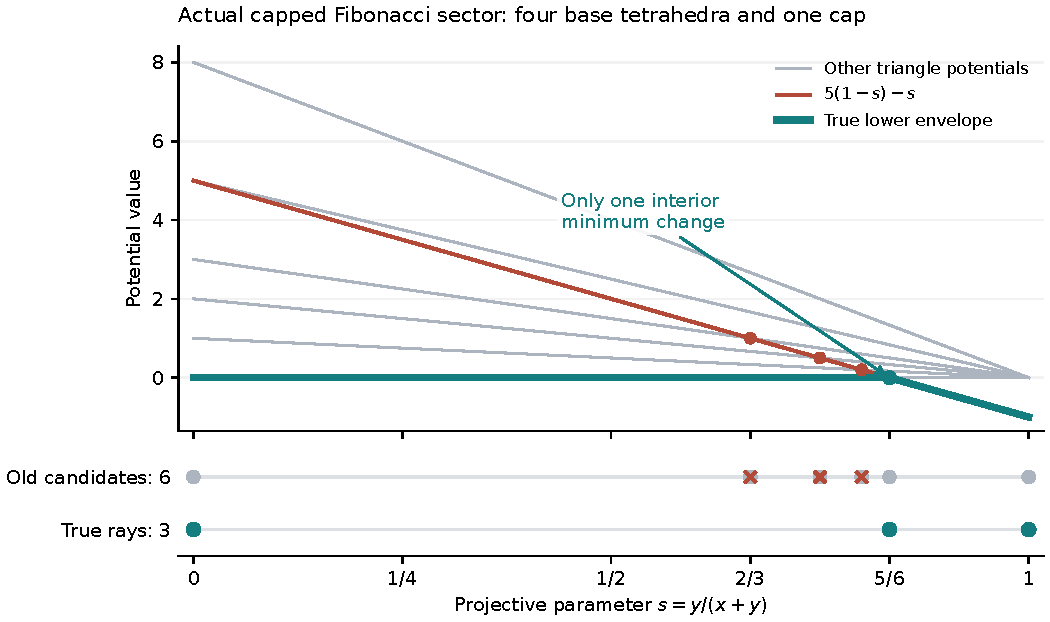
\includegraphics[width=\linewidth]{figures/minimum_envelope.pdf}
\caption{The actual potential functions for the capped family with $n=4$,
using the positive projective normalization $x+y=1$. Three interior
pairwise crossings fail to change the minimum and give no standard ray.
The true change at $s=5/6$, together with the endpoints, gives all three
rays. The lower strip marks the complete old candidate list and the exact
new output list.}
\label{fig:envelope}
\end{figure}

\begin{corollary}[Exact surplus in the old arrangement]
\label{cor:oldfamily}
For this family, the old arrangement has $n+3$ distinct projected hyperplanes,
$n+2$ nonzero nonnegative candidate directions, and $n-1$ nonextreme
directions that are rejected. The envelope method emits exactly three rays.
\end{corollary}

\begin{proof}
Modulo a common old-vertex potential, the distinct potential forms are
\[
 0,\ F_2x,\ F_3x,\ldots,F_{n+2}x,\ A_nx-y.
\]
The new vertex contributes no differences. Equalities between pure
multiples of $x$ all give $x=0$. The remaining equalities give
$y=(A_n-c)x$ for
$c\in\{0,F_2,F_3,\ldots,F_{n+2}\}$. There are $n+2$ distinct such
slopes, exactly one negative, arising from $c=B_n>A_n$. The quadrilateral
coordinate hyperplanes add none: $x=0$ already occurs and $y=0$ is the
case $c=A_n$. Thus there are $n+3$ distinct hyperplanes, of which $n+2$
give nonnegative directions. Theorem~\ref{thm:family} leaves only three
standard rays, so $n-1$ positive directions fail extremality. Their
intermediate equalities do not change the true minimum.
\end{proof}



For $n=1$, the three rows of the following table give the complete output.
The separating semicolon distinguishes triangles from quadrilaterals. The
second ray has an independently replayable disc certificate in
\texttt{examples/extra\_non\_q\_disc.json}.

\begin{table}[ht]
\centering\small
\begin{tabular}{@{}ccl@{}}
\toprule
$(x,y)$ & Original tetrahedron; cap tetrahedron & Topology\\
\midrule
$(1,0)$ & $(1,1,0,0;0,0,1)$; $(1,2,0,0;0,0,0)$ & Essential disc\\
$(1,1)$ & $(1,1,0,0;0,0,1)$; $(0,2,0,0;0,1,0)$ & Essential disc\\
$(0,1)$ & $(1,1,1,1;0,0,0)$; $(0,1,0,1;0,1,0)$ & Inessential disc\\
\bottomrule
\end{tabular}
\caption{The smallest capped-family sector. The interior standard ray is
absent from the quadrilateral vertex list.}
\end{table}

The formulas also give a direct family-specific oracle using $O(n)$
Fibonacci additions and coordinate operations. The complete output has
$\Theta(n^2)$ bits because it contains a linear sequence of Fibonacci
coordinates of linearly growing binary lengths. Standard binary addition
evaluates the formulas in $O(n^2)$ bit time. The delivered generic kernel
builder is not replaced by a special recognizer for this family; the formulas
serve as a separate mathematical description and are implemented as an oracle
in \texttt{experiments/family\_oracle.py}.


The example does not claim that the endpoints fail every useful recognition
test. In fact the recorded small family also has an essential disc at one
endpoint. Its role is to show that the complete output query is stronger
than a first-witness query, and to exhibit a large cost of the previous
implementation on genuine finite triangulations. The control cap type has
no genuine interior change and only two standard rays; it is included to
measure the cost when there is less spurious work to remove.

\section{Certified reduction to an effective small face}
\label{sec:facialreduction}

The implementation dispatches on rational nullity at most two. The geometric
theorem itself only needs a projective section of dimension at most one.
The following elementary certificate can extend applicability after additional
preprocessing; automatic production of these certificates is not part of the
new code.

\begin{proposition}[Certified zero-coordinate reduction]
\label{prop:zeros}
Suppose a rational row vector $y$ satisfies $z=y^TA\ge0$. Every vector
$q\in\cone$ has $q_i=0$ whenever $z_i>0$. Deleting those allowed coordinates
leaves exactly the same standard sector cone, with zeros reinserted. If a
sequence of such certified reductions leaves matching nullity at most two,
the envelope theorem gives a complete ray list for the original sector.
\end{proposition}

\begin{proof}
For $q\in\cone$, $0=y^TAq=zq=\sum_i z_iq_i$. Each summand is nonnegative,
so every summand with $z_i>0$ has $q_i=0$. Removing coordinates already forced
to zero changes neither the matching solutions nor their standard lifts.
The same argument applies successively, and coordinate-face identification
preserves the complete standard ray set.
\end{proof}

This is a sufficient certified extension, not a claim that checking individual
cycle-row signs finds every forced zero. Linear combinations whose resulting
row is nonnegative may reveal zeros that individual rows miss. Exact dual certificates and
propagation from the incoming linear-programming work are natural sources
for such reductions.\cite{incomingdual} Constructing a complete and efficient
relative-interior support reduction, and measuring its benefit before envelope
enumeration, is a concrete next implementation task.

\section{Implementation and integration contract}
\label{sec:implementation}

The new modules use only the Python standard library. Regina is an optional
independent oracle for experiments; it is not called by the producer or the
certificate checker. Exact integers and \texttt{fractions.Fraction} are used
throughout. No floating-point decision determines feasibility, equality,
breakpoint order, primitive scaling, or completeness.

\begin{table}[htbp]
\centering
\begin{tabular}{@{}>{\raggedright\arraybackslash}p{6.1cm}>{\raggedright\arraybackslash}p{8.1cm}@{}}
\toprule
Module or artifact & Responsibility\\
\midrule
\texttt{sector\_envelope.py} & Feasible projective section, exact lower
envelopes, cached lifts, and the complete ray iterator.\\
\texttt{sector\_envelope\_certificate.py} & Compact coverage-certificate
production and a capped complete-enumeration API.\\
\texttt{sector\_envelope\_verify.py} & Independent uncontracted source
reconstruction, dimension check, slope-bracket replay, and full-list checking.\\
\texttt{normal\_sector.py} & A small integration change adds the explicit
\texttt{method='envelope'} option for standard enumeration and forwards the
method through the supplied-sector discovery API.\\
\texttt{tests/test\_sector\_envelope*.py} & Algebra, geometric comparisons,
malformed certificates, budget boundaries, and producer-disabled replay.\\
\texttt{sector\_envelope\_research/} & Declared corpus audit, actual
triangulation generators, paired timing experiments, and supporting data.\\
\bottomrule
\end{tabular}
\caption{Implementation modules and their responsibilities. The supplied
snapshot also retains their maintained dependencies.}
\end{table}

The option is explicit. Existing \texttt{auto}, \texttt{arrangement}, and
\texttt{supports} choices retain their earlier selection rules; the
quadrilateral phase also retains its earlier path. The patch therefore does
not silently introduce a full standard-ray enumeration into the recognizer's
first-witness route. It offers a faster complete query where its hypotheses
are checked. Matching nullity above two is rejected by this method, allowing
a caller to choose another exact backend.

\begin{lstlisting}[language=Python,caption={Complete enumeration and independent replay.}]
from fastunknot.sector_envelope_certificate import certify_sector_enumeration
from fastunknot.sector_envelope_verify import verify_sector_envelope_certificate

answer = certify_sector_enumeration(triangulation, allowed_types, max_rays=None)
assert answer['status'] == 'COMPLETE'
assert verify_sector_envelope_certificate(triangulation, answer['certificate'])
# answer['coordinates'] is the full non-link standard-ray list in this sector.
\end{lstlisting}

\subsection{Caps and cancellation}

In the envelope iterator, \texttt{max\_bases} counts output candidates whose
full lift has begun; there are no redundant arrangement bases in this branch.
If a cap is reached before the next candidate, the existing
\texttt{SearchLimit} exception is raised. A partial iterator is not an
absence certificate. The coverage-producing API checks its \texttt{max\_rays}
allowance against the planned complete list and returns
\texttt{INCONCLUSIVE} without a certificate if it is insufficient.

The same numeric cap can thus permit different progress in the old and new
methods, which is expected: their work units differ. Tests use uncapped
complete queries for equality claims. Callback cancellation is propagated
by identity, including false-valued callable objects and exceptions whose
classes coincide with internal limit or geometry exceptions. Hexadecimal
integer transport handles large exact fields without altering process-wide
decimal conversion limits.

\section{Validation and measured performance}
\label{sec:experiments}

\subsection{Correctness evidence}

The main regression run completed 1,334 tests successfully in 144.558 seconds
on CPython 3.12.14. Three additional focused producer tests were subsequently
added for multiple vertex groups, multiple genuine changes, and endpoint-only
ties; the final focused run completed all 24 producer and certificate tests.
Its result is recorded separately in the accompanying test log. This avoids attributing those later test additions to the earlier
full-suite run.

The host reports an AMD EPYC 9V74 processor under Linux on x86-64.
\path{results/environment.json} records the runtime and dependency
versions. The paired measurements use elapsed wall time; the processor's
model name is not a claim of exclusive access to the host.

\begin{table}[ht]
\centering
\begin{tabular}{@{}lr@{}}
\toprule
Check & Completed instances\\
\midrule
Full maintained regression suite & 1,334\\
Final focused producer and certificate tests & 24\\
Frozen finite triangulations represented & 48\\
Declared selected sectors & 9,995\\
Eligible sectors with matching nullity at most two & 9,344\\
Higher-nullity sectors transparently outside the new branch & 651\\
Emitted ray occurrences compared with the complete frozen oracle & 4,853\\
Interior standard-ray occurrences in those comparisons & 804\\
Empty feasible cones correctly returned & 6,276\\
Fresh Regina complete standard enumerations & 15\\
Independent graph-versus-dense model comparisons & 66\\
Complete certificates in the separate source-model audit & 60\\
Family sizes checked against the closed-form ray oracle & 9\\
Integral family vectors with checked component topology & 97\\
\bottomrule
\end{tabular}
\caption{Validation counts. Ray counts are occurrences over the selected
queries, not counts of globally distinct surfaces. All stated comparisons
agreed. The six model-only cases had higher nullity.}
\end{table}

\begin{table}[ht]
\centering
\begin{tabular}{@{}lrrrr@{}}
\toprule
Matching nullity & Queries & Empty section & Point section & Interval section\\
\midrule
0 & 5,357 & 5,357 & 0 & 0\\
1 & 2,837 & 890 & 1,947 & 0\\
2 & 1,150 & 29 & 140 & 981\\
\bottomrule
\end{tabular}
\caption{Feasible-section stratification. In particular, nullity two does
not guarantee a nondegenerate interval.}
\end{table}

The corpus selects supports occurring in recorded standard or quadrilateral
rays, every support with at most two allowed types, and 64 fixed-seed full
sectors for each triangulation. For triangulations with at most three
tetrahedra, it selects every compatible support. The union is deduplicated
before testing. Larger triangulations are not claimed to have had every one
of their exponentially many sectors tested. The frozen corpus SHA-256 and
source pins are retained in \texttt{results/audit.json}.

The 15 fresh Regina runs comprise six original corpus fixtures and nine
capped-family inputs with base sizes 1, 2, and 4 and each of the three cap
types. Regina reports runtime version 7.4; its installed Python distribution
is version 7.4.1.\cite{regina} The new producer and checker use no Regina
calls. In the separate independent audit, 66 models across all 48 original
triangulations were reconstructed both from the uncontracted graph and by
dense standard matching elimination. Their nullspaces and all relative
vertex potentials agreed; all 60 eligible complete certificates replayed.

The affine hull tests use 120 fixed-seed rational line sets and compare
against literal minima at every pairwise crossing and points in the intervening
intervals, giving over 5,000 exact sample comparisons. They also cover
a rational basis change with denominator $2^{257}+7$ (258 bits). These checks are paired with complete
geometric ray-list comparisons, so a correct hull routine alone is not
treated as evidence for an incorrect normal-surface reduction.

The separate family oracle evaluates the closed coordinate formulas without
calling the matching kernel or envelope routine. Its ray lists agree at
base sizes $1,2,3,4,8,16,32,64,128$. At the first five sizes it also checks
the old hyperplane and rejected-direction counts. For base sizes
$1,2,4,8$, it checks 97 integral vectors with parameters on both sides of
the hinge, including the hinge itself. The native compressed component
census and its independent certificate replay give exactly $x+h$ components
and $x$ essential discs in every case. These finite checks supplement the
all-size proof; they do not substitute for it.

\subsection{Controlled complete-enumeration measurements}

The retained experiment has 13 geometric cohorts, one warm-up per scope,
and five paired rounds in alternating AB/BA order. The eight-tetrahedron
base with cap type one also has duplicate same-method A/A arms. There are
280 measured calls and 52 warm-up calls across the two scopes, followed by
three new-method-only capacity runs. The immutable predecessor is copied
from the pinned repository revision, rather than recreated by editing the
optimized implementation. Every measured output hash agrees between arms,
and the timed source-file hashes are checked before and after the run.

Table~\ref{tab:enumeration} reports medians in milliseconds. Its speedup is
the median of the five \emph{paired ratios}, which need not equal the ratio
of the two separately reported medians. The last column isolates enumeration
with an already constructed kernel. Full raw calls, order, setup costs,
work counters, and source hashes are in \texttt{results/benchmark.json}.

\begin{table}[htbp]
\centering\small
\begin{tabular}{@{}rrrrrr@{}}
\toprule
$t$ & Cap & Old full (ms) & New full (ms) & Full speedup & Reused speedup\\
\midrule
2 & 1 & 0.626 & 0.425 & 1.51$\times$ & 2.02$\times$\\
2 & 2 & 0.550 & 0.324 & 1.75$\times$ & 2.28$\times$\\
5 & 1 & 8.020 & 1.021 & 7.85$\times$ & 13.88$\times$\\
5 & 2 & 7.516 & 0.993 & 7.70$\times$ & 13.00$\times$\\
9 & 1 & 56.963 & 2.548 & 22.89$\times$ & 41.01$\times$\\
9 & 2 & 75.142 & 2.603 & 30.59$\times$ & 45.10$\times$\\
17 & 1 & 476.595 & 6.921 & 68.86$\times$ & 167.84$\times$\\
17 & 2 & 526.057 & 9.083 & 66.86$\times$ & 171.14$\times$\\
33 & 1 & 6,063.538 & 29.023 & 202.71$\times$ & 781.17$\times$\\
33 & 2 & 6,308.664 & 30.404 & 207.49$\times$ & 728.34$\times$\\
\midrule
9 & 0 & 17.964 & 2.119 & 8.07$\times$ & 17.00$\times$\\
17 & 0 & 98.115 & 7.708 & 12.62$\times$ & 35.20$\times$\\
33 & 0 & 569.414 & 28.207 & 19.75$\times$ & 75.50$\times$\\
\bottomrule
\end{tabular}
\caption{Complete enumeration on capped Fibonacci solid tori. Here
$t=n+1$ includes the cap. ``Full'' includes kernel construction and full
standard-coordinate emission. Types one and two have three rays; type zero
is the two-ray control. Every query has matching nullity two.}
\label{tab:enumeration}
\end{table}

For $t=33$ and cap type one, the old and new full medians are
6.064 seconds and 29.023 milliseconds, with paired speedup $202.71\times$.
The reused-kernel medians are 6.593 seconds and 8.204 milliseconds,
with paired speedup $781.17\times$. These are local complete-enumeration
measurements on the declared family, not whole-recognizer measurements.

The growth in redundant work is also visible without a clock. At base size
$n=32$, the old backend constructs 35 distinct hyperplanes, tries 34
nonnegative directions, and rejects 31; the new method lifts precisely three
directions. Corollary~\ref{cor:oldfamily} proves these counts for every
size. The timing difference also includes the cost of constructing pairwise
forms and applying dense supported-rank tests, so it should not be explained
only by the ratio of candidate counts.

The same-method duplicate ratios (first call divided by duplicate) have medians 0.969 and 0.974 for reused old/new calls, and 0.794 and 1.037 for full old/new calls. This visible host variability argues against treating small differences or last decimal places as reliable. No confidence interval or power-law fit is claimed.


\begin{table}[htbp]
\centering\small
\begin{tabular}{@{}rrrrr@{}}
\toprule
$t$ & Kernel (ms) & Enumeration (ms) & Total (ms) & Kernel share\\
\midrule
65 & 126.833 & 28.028 & 154.861 & 81.9\%\\
129 & 926.795 & 144.873 & 1,071.667 & 86.5\%\\
257 & 7,493.208 & 395.727 & 7,888.936 & 95.0\%\\
\bottomrule
\end{tabular}
\caption{New-method-only capacity runs with cap type one and three emitted
rays. Each row is a single call, not a paired comparison or a median.}
\label{tab:capacity}
\end{table}

At $t=257$, approximately 95\% of the new full call is kernel construction.
This identifies a concrete implementation target after removing arrangement
work. The capacity rows do not imply a measured speedup at these sizes:
the predecessor was not run there.

\begin{figure}[htbp]
\centering
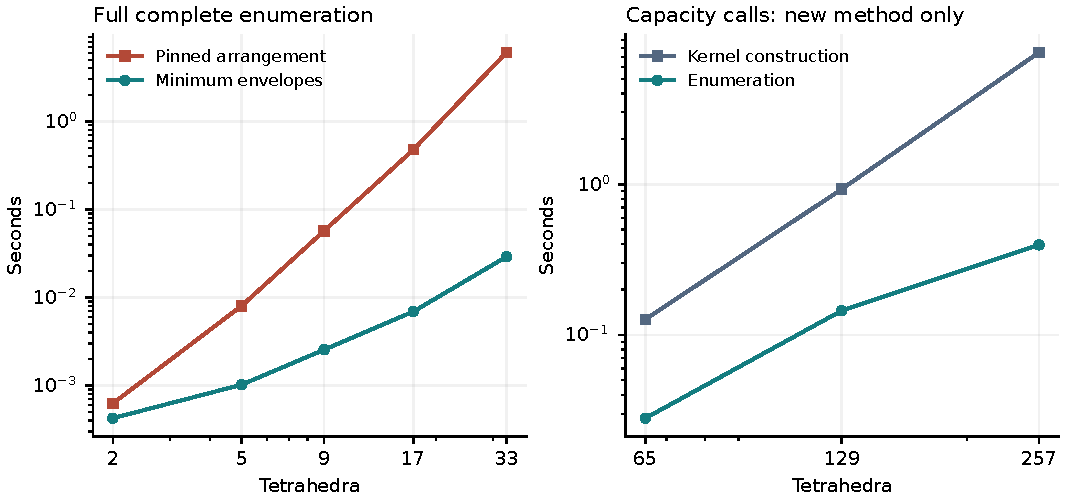
\includegraphics[width=\linewidth]{figures/measurements.pdf}
\caption{Measured complete-enumeration times. Left: five-round medians of
full calls on cap-type-one inputs, including kernel construction. Right:
the three new-method-only capacity calls, separated into kernel and
enumeration time. Both axes in each panel are logarithmic. Lines connect
observations and are not fitted complexity laws.}
\label{fig:measurements}
\end{figure}

\subsection{Production followed by independent coverage checking}

A separate matched workflow includes completeness checking. The old arm
constructs the pinned kernel, enumerates with the pinned arrangement, then
reconstructs the independent dense matching model and runs its complete
reference enumeration to check equality. The new arm produces an envelope
coverage certificate and replays it with the independent uncontracted-graph
checker. Both workflows require the same complete ray list. The new API
constructs its plan for both production and certification; this duplicate
constant-factor work is included in the timings.

There is one warm-up and three paired AB/BA rounds for each compared size.
Fixture generation and final reporting serialization and hashing are outside
the timed regions. The old arm's ray-list equality check and the new arm's
certificate verification, including their internal hashes, are included.
\texttt{results/coverage.json} retains every call, source hash, and six
independently replayable source/certificate pairs.

\begin{table}[htbp]
\centering\small
\begin{tabular}{@{}rrrr@{}}
\toprule
$t$ & Old production + replay (ms) & New production + replay (ms) & Paired speedup\\
\midrule
2 & 1.713 & 1.010 & 1.68$\times$\\
9 & 130.931 & 8.628 & 15.18$\times$\\
17 & 1,326.585 & 29.259 & 51.92$\times$\\
\bottomrule
\end{tabular}
\caption{Complete production and independent coverage, cap type one.
Reported times are medians; speedups are medians of paired ratios.}
\label{tab:coveragebench}
\end{table}

\begin{table}[htbp]
\centering\small
\begin{tabular}{@{}rrrrrr@{}}
\toprule
$t$ & Production (ms) & Replay (ms) & Total (ms) & Certificate bytes & Tests\\
\midrule
33 & 43.729 & 53.800 & 97.529 & 3,915 & 132\\
65 & 248.320 & 328.658 & 576.978 & 9,985 & 260\\
129 & 1,616.358 & 2,322.612 & 3,938.970 & 29,654 & 516\\
\bottomrule
\end{tabular}
\caption{New-only production and coverage capacity calls. ``Tests'' counts
slope-bracket dominance checks, exactly $4t$ per row. Each list has three
rays. JSON sizes include the complete coordinates; serialization is untimed.}
\label{tab:coveragecapacity}
\end{table}

The coverage workflow at $t=17$ has median paired speedup $51.92\times$;
its three ratios range from $34.61\times$ to $60.72\times$. This broader
scope shows that the benefit persists after checking a complete answer.
At $t=129$, new production and replay take a single combined 3.939 seconds;
this is a capacity observation without a comparative claim. The $4t$
dominance count does not imply a linear-time full checker, since matching
elimination, projection, and coordinate validation must also be performed.



The audit distinguishes a test method from the thousands of mathematical
instances checked inside it. The frozen-corpus selection rule is encoded in
the script before results are classified: it is not a list chosen after
observing which sectors are fast. Comparisons filter a complete standard-ray
oracle by allowed quadrilateral support, which is valid because the sector
is a coordinate face. Pure vertex links are removed from both lists.

Fresh oracle comparisons use Regina's own complete standard enumeration on
small declared inputs. They complement, rather than replace, the broader
frozen comparisons. Random affine-line tests inspect every pairwise crossing
and points in the intervening intervals; they are a check of the hull
implementation, whereas the finite-triangulation comparisons test the
mathematical connection to normal surfaces.

Timing comparisons use the same exact output query and verify equality of
primitive ray sets. Reused-kernel measurements isolate enumeration; rebuild
measurements include construction of the matching kernel. Complete coverage
measurements additionally run the independent checker. Output multiplicity
is never expanded into individual discs for either timing arm.

Ratios are descriptive measurements, not complexity proofs. Repeated rounds
and alternating order reduce simple timing bias but do not make the hardware
or Python runtime universal. The ordinary recognizer does not automatically
call the new complete-sector method, so this report has no measured
end-to-end knot-recognition speedup or increase in its recognition coverage.

\section{What follows for quasi-polynomial recognition}
\label{sec:global}

The local result is useful even for dense supports: $k$ can be proportional
to $t$, and primitive disc coordinates can be exponentially large. The
condition concerns the residual matching dimension, not a logarithmic bound
on the number of occupied tetrahedra. This avoids the universal sparse-support
assumption already contradicted by layered meridians in the previous sector
work.\cite{report57}

It does not bound how many sectors must be discovered. A fast observer of a
supplied normal vector, a fast first positive-Euler query, and a fast complete
enumerator inside one specified sector each address different parts of the
problem. Only a source-bound construction with a coverage argument can turn
those local tools into a complete recognition algorithm.

\begin{theorem}[Conditional complete-family bound]
\label{thm:conditional}
Suppose a deterministic procedure on an $n$-crossing knot diagram constructs
at most $S(n)$ supplied finite sectors, possibly after certified transformations,
and the following properties hold:
\begin{enumerate}
\item Source correspondence and every topology transformation are certified
and preserve the recognition problem under the stated terminal rules.
\item Every generated sector has polynomial encoded size in $n$ and matching
nullity at most two, or is reduced to such a sector by checked zero-coordinate
certificates.
\item Construction and all auxiliary work, including unsuccessful branches,
restarts, and terminal checks, cost $S(n)\poly(n)$ in total.
\item For every generated normal vector, a deterministic procedure computes
the required component and essential-disc predicates, produces the
corresponding source-bound certificates, and replays them in time polynomial
in the original diagram size $n$, under the actual terminal hypotheses of
the strategy.
\item If the original diagram is an unknot, at least one of the enumerated
standard rays contains the required certified compressing-disc witness;
the negative conclusion from complete exhaustion is justified by this
coverage statement and the source correspondence.
\end{enumerate}
Then complete enumeration and certified disc search over this family can be
performed in $S(n)\poly(n)$ bit time. In particular, if
$S(n)\le n^{O(\log n)}$, the resulting algorithm has that same asymptotic
bound.
\end{theorem}

\begin{proof}
Theorems~\ref{thm:count} and~\ref{thm:cost} give polynomially many
polynomial-size candidates in each sector, with polynomial encoded generation
cost. Primitive-coordinate size is bounded by Lemma~\ref{lem:height}, and
the independent coverage check is polynomial by
Theorem~\ref{thm:coverage}. Applying the deterministic compressed component
procedure in the fourth hypothesis adds polynomial time per candidate,
including production and replay of the required source-bound certificates.
The hypotheses bound all other work and justify both the positive and
negative conclusions. Summing over the at most $S(n)$ sectors yields the
claim.
\end{proof}

The final coverage hypothesis is not established here. It is not enough that many
experimental discs happen to lie in small-dimensional sectors. The other
hypotheses likewise require costs in the original diagram size, not
only in the size of an uncontrolled intermediate triangulation. If a
hierarchy generates a tree of states, $S(n)$ must include all explored nodes
and abandoned suffixes. Polynomial branching through $O(\log n)$ levels
gives the desired $n^{O(\log n)}$ count. Replacing that depth by
$O(\log^2 n)$ yields a different exponent and cannot be silently conflated
with the stated target.

\subsection{A precise next milestone}

A useful next target is a certified procedure that selects a useful surface
from a small-dimensional sector and carries out one complete topology
transition, including the ordered boundary attachments needed to continue.
The new result supplies complete local alternatives and a checkable
exhaustion record for that selection. It still needs a selection policy, an
embedding-aware continuation test, and a potential controlling how often
the state must be changed or revisited.

\section{Further research questions and priorities}
\label{sec:research}

\begin{enumerate}[label=\textbf{\arabic*.},leftmargin=*]
\item \textbf{Certified effective-dimension reduction.}
Implement production of Proposition~\ref{prop:zeros} certificates from the
incoming dual solver. Measure how often raw nullity above two falls to two
on the relative interior support. Compare the complete cost of reduction and
enumeration against the current arrangement, rather than reporting the
dimension decrease alone.

\item \textbf{Minimum subdivisions in dimension three.}
For matching nullity three the normalized domain is a polygon. Develop an
exact traversal of its actual minimum subdivision, including boundary
vertices and coincident faces. The fan theorem removes rank filtering once
these vertices are certified, but the arrangement can no longer be replaced
by a one-dimensional event merge. Establish explicit output and intermediate
complexity bounds for a carefully specified representation.

\item \textbf{A geometric bound on complete sector families.}
Find a deterministic family of low-dimensional sectors that covers a
compressing-disc witness whenever one exists in the relevant knot-exterior
class. Identify which triangulation or hierarchy restrictions make such a
claim plausible. A bound on the number of sectors is more valuable to the
global goal than another improvement to a fixed supplied vector.

\item \textbf{Surface choice using complete alternatives.}
The extra interior standard rays can have useful topology. Design a
component-aware objective that chooses among all rays using essentiality,
boundary order, and the complexity of the subsequent cut. A first positive
Euler value is insufficient to define this objective. Preserve explicit
counterexamples where Euler or aggregate boundary tests discard necessary
information.

\item \textbf{Incremental kernels under certified local moves.}
The envelope stage can become much cheaper than rebuilding the matching
kernel. Track how cycle rank, potentials, and active hulls change under the
already certified local triangulation operations. Reuse only data whose
source correspondence is checked; otherwise a fast stale envelope is an
incorrect one.

\item \textbf{Persistent coverage certificates.}
Determine whether unchanged vertex envelopes can retain their certificates
across a local modification. A valid approach must transport corner names,
projective parameters, and matching-space information. Prove an amortized
bound for all required invalidations, not just successful reuse cases.

\item \textbf{Compressed output and streaming topology.}
Full $7t$ vectors impose an $\Omega(tN)$ output requirement. Couple the
projected-lift representation directly to the compressed component observer
while keeping an independently checkable source binding. This could save
repeated coordinate scans, but should not hide the cost of any requested
full output vectors.

\item \textbf{Sharp geometric ray counts.}
Is $3k+4$ asymptotically sharp for realizable finite-manifold sectors with
matching nullity two? The abstract lower-envelope construction only shows
sharpness of the piece-count expression. Construct a geometric linear lower
bound, or exploit additional normal-matching structure to improve the
coefficient or the dependence on the number of vertex groups.

\item \textbf{Oracle-independent topology validation.}
Extend the certificate boundary so that triangulation validity and the
diagram-to-exterior construction have independent native replay. The present
checker is independent of enumeration, but deliberately shares some native
geometry validation with the producer. This is a concrete trust-boundary
improvement distinct from faster ray generation.

\item \textbf{Whole-search accounting.}
Use the new complete local query inside one specified recognition strategy
and record every unsuccessful sector, cutoff, repeated state, and topology
repair. Seek a decreasing or amortized potential in original-input size.
Any quasi-polynomial claim must bound that complete trace, not only the
number of successful hierarchy stages.
\end{enumerate}

\appendix
\section{Certificate schema and adversarial checks}
\label{app:schema}

The schema identifier is \texttt{normal-sector-envelope-v1}. It binds the
triangulation by its canonical JSON SHA-256 digest and includes an ordered
allowed-type list. Exact rational values are reduced numerator--denominator
pairs with a positive denominator. Large integer fields can use the
repository's explicit signed hexadecimal representation.

The checker accepts exactly the stated sector coverage claim, not arbitrary
metadata attached to it. It verifies the independently recovered matching
dimension; emptiness or exact projective bounds; an anchor chain for every
global vertex in a nondegenerate section; one checked slope bracket for each
original corner; and the complete ordered list of primitive canonical lifts.
Matching dimensions above two are outside this schema's accepted method.

Mutation tests cover a changed source hash, omitted or additional ray,
incorrect coordinate, false matching dimension, shortened interval,
noncanonical rational, missing or duplicated vertex record, wrong active
corner, missing dominance hint, and an incorrect bracket. A specially
constructed affine-line adversary places an omitted line below the claimed
chain between its endpoints; the slope-bracket test rejects it. Merely
checking the global interval endpoints would miss such an undercut.

The producer-disabled test replaces the new enumeration and hull functions,
the sector-kernel builder, and reference ray enumerators with functions that
raise if called. A previously generated valid certificate still replays.
This tests an actual independence boundary, rather than merely checking that
the producer agrees with itself.

\section{Reproduction and integration}
\label{app:reproduction}

The archive includes a self-contained source snapshot for the focused
experiments, the exact predecessor of the changed sector dispatcher, a patch
against the pinned repository, declared fixtures, raw measurements, and this
article's source. The top-level \texttt{README.md} gives the current commands
and explains quick and full reproduction. Optional Regina checks require the
recorded Regina version; the production code and focused native certificate
tests need only the standard library.

The integration patch adds the new modules and research/test files and changes
only the supplied-sector method dispatch in maintained code. It does not
modify the repository's historical reports, apply other incoming patches, or
replace the recognizer's default strategy. Applying it to a different revision
requires the ordinary review of overlapping changes. The patch is supplied
for integration; no remote repository mutation is part of this delivery.

The recorded full-suite result applies to the pinned checkout plus this
patch in the recorded runtime. The broad corpus result counts the selected
eligible sectors tested, not every sector of every possible triangulation.
The timing result concerns the exact queries named in the tables. These
three statements should remain separate when the work is incorporated into
the maintained synthesis.

\clearpage
\section{Claim ledger}

{\small
\begin{longtable}{@{}>{\raggedright\arraybackslash}p{5.7cm}>{\raggedright\arraybackslash}p{2.7cm}>{\raggedright\arraybackslash}p{5.8cm}@{}}
\toprule
Claim & Status & Evidence or limitation\\
\midrule\endhead
Anchored minimum cells are coordinate faces under canonical lifting.
& Proved & Theorem~\ref{thm:fan}, all dimensions.\\
Endpoints and genuine lower-envelope changes enumerate every standard ray
when matching nullity is at most two.
& Proved & Theorem~\ref{thm:envelope}, including empty and singleton sections.\\
$N\le p-g+2\le3k+4$ in the nondegenerate nullity-two case.
& Proved & Cycle-rank argument and Theorem~\ref{thm:count}.\\
Primitive coordinate bound $4^k$.
& Inherited; reproved & Mixed-column minors, Lemma~\ref{lem:height}; preceding
sector work.\\
Post-kernel enumeration has the stated polynomial encoded cost.
& Proved & Theorem~\ref{thm:cost}; kernel, validation, and full output charged.\\
One slope-bracket test per original line certifies complete envelope coverage.
& Proved & Lemma~\ref{lem:bracket}, Theorem~\ref{thm:coverage}.\\
The implementation produces the declared oracle ray lists.
& Checked & Frozen corpus, fresh Regina checks, and focused
independent comparisons.\\
Measured speedups on the declared capped layered-torus queries.
& Measured & Paired raw timings; query and preprocessing scope stated.\\
More diagrams are recognized, or ordinary recognition is faster.
& Not established & The new complete-sector method is explicit and is not
automatically invoked by the default recognizer.\\
A complete $n^{O(\log n)}$ algorithm for arbitrary knot diagrams.
& Open in this work & Missing complete family and transformation bounds;
Theorem~\ref{thm:conditional} states the required hypotheses.\\
\bottomrule
\end{longtable}
}

\clearpage
\begin{thebibliography}{99}
\bibitem{burtonconversion}
Benjamin A. Burton, \emph{Converting between quadrilateral and standard
solution sets in normal surface theory}, Algebraic \& Geometric Topology
\textbf{9} (2009), 2121--2174.
\href{https://doi.org/10.2140/agt.2009.9.2121}{doi:10.2140/agt.2009.9.2121};
\href{https://arxiv.org/abs/0901.2629}{arXiv:0901.2629}.

\bibitem{burtonfaces}
Benjamin A. Burton, \emph{Maximal admissible faces and asymptotic bounds for
the normal surface solution space}, Journal of Combinatorial Theory,
Series A \textbf{118} (2011), 1410--1435.
\href{https://doi.org/10.1016/j.jcta.2010.12.011}{doi:10.1016/j.jcta.2010.12.011};
\href{https://arxiv.org/abs/1004.2605}{arXiv:1004.2605}.

\bibitem{burtonozlen}
Benjamin A. Burton and Melih Ozlen, \emph{A fast branching algorithm for
unknot recognition with experimental polynomial-time behaviour},
Mathematical Programming \textbf{164} (2017), 283--308.
\href{https://arxiv.org/abs/1211.1079}{arXiv:1211.1079}, version 3.

\bibitem{treetraversal}
Benjamin A. Burton and Melih Ozlen, \emph{A tree traversal algorithm for
decision problems in knot theory and 3-manifold topology}, Algorithmica
\textbf{65} (2013), 772--801.
\href{https://arxiv.org/abs/1010.6200}{arXiv:1010.6200}, version 2.

\bibitem{cgalenvelopes}
Ron Wein, \emph{2D Envelopes}, CGAL User and Reference Manual, version 6.2.
\url{https://doc.cgal.org/6.2/Envelope_2/index.html}. Accessed 9 October 2026.

\bibitem{lackenby2026}
Marc Lackenby, \emph{Incompressible surfaces, hierarchies and unknot
recognition}, preprint, 25 July 2026.
\href{https://arxiv.org/abs/2607.23350}{arXiv:2607.23350}, version 1.

\bibitem{regina}
The Regina development team, \emph{Regina: software for low-dimensional
topology}, runtime version 7.4 (Python distribution 7.4.1) used for the fresh
checks in this package.
\url{https://regina-normal.github.io/}.

\bibitem{repo}
Vladimir Reshetnikov, \emph{ProveIt: Topology/UnknotRecognition}, repository
snapshot \texttt{66098968e88bba797143ac1bf7ad0ac4c5f697df}, 9 October 2026.
\href{https://github.com/VladimirReshetnikov/ProveIt/tree/66098968e88bba797143ac1bf7ad0ac4c5f697df/Topology/UnknotRecognition}{Pinned GitHub source snapshot}.

\bibitem{report57}
ProveIt research archive, \emph{Quadrilateral Support Kernels and Certified
Normal-Disc Discovery}, Report 57, 9 October 2026. Maintained implementation:
\texttt{fast/fastunknot/normal\_sector.py}; independent model:
\texttt{normal\_sector\_verify.py}; frozen corpus:
\texttt{reports/57/results/discovery\_corpus.json}, at the repository snapshot
in~\cite{repo}.

\bibitem{incomingdual}
ProveIt incoming research package,
\texttt{unknot\_dual\_certificates\_20261009.zip}, particularly the setting,
sector linear-programming, propagation, and further-research sections.
\texttt{docs/incoming/}, at the repository snapshot in~\cite{repo}.

\bibitem{incomingsupport}
ProveIt incoming research package,
\path{unknot_support_sensitive_certificates_20261009.zip}.
\texttt{docs/incoming/}, at the repository snapshot in~\cite{repo}.

\bibitem{incomingtransport}
ProveIt incoming research package,
\texttt{unknot\_geometric\_transport\_20261009.zip},
\emph{Cocycle Transport and Ordered Boundary Interfaces for Unknot Recognition}.
\texttt{docs/incoming/}, at the repository snapshot in~\cite{repo}.
\end{thebibliography}
\end{document}
